\documentclass[10pt]{book}
\usepackage{gvv-book}
\usepackage{gvv}
\usepackage[sectionbib,authoryear]{natbib}% for name-date citation comment the below line
\usepackage{setspace}
\setstretch{1.0}
%\usepackage[sectionbib,numbers]{natbib}% for numbered citation comment the above line
%%********************************************************************%%
%%       How many levels of section head would you like numbered?     %%
%% 0= no section numbers, 1= section, 2= section, 3= subsection %%
\setcounter{secnumdepth}{3}
%%********************************************************************%%
%%**********************************************************************%%
%%     How many levels of section head would you like to appear in the  %%
%%				Table of Contents?			%%
%% 0= chapter, 1= section, 2= section, 3= subsection titles.	%%
\setcounter{tocdepth}{2}
%%**********************************************************************%%
%\includeonly{ch01}
\makeindex
\let\cleardoublepage\clearpage
\begin{document}
\frontmatter
%%%%%%%%%%%%%%%%%%%%%%%%%%%%%%%%%%%%%%%%%%%%%%%%%%%%%%%%%%%%%%%%
\booktitle{Geometry}
\subtitle{Through Algebra}
\AuAff{Errala Paulsonashish}
%\halftitlepage
\titlepage
\tableofcontents
%\listoffigures %optional
%\listoftables  %optional
%% or Contributor Page for edited books
%% before \tableofcontents
%%%%%%%%%%%%%%%%%%%%%%%%%%%%%%%%%%%%%%%%%%%%%%%%%%%%%%%%%%%%%%%%
\setcounter{page}{0}
\begin{introduction}
This book shows how to solve problems in geometry using trigonometry and coordinate geometry. 
\end{introduction}
\mainmatter
\chapter{Triangle}
Consider a triangle with vertices
		\begin{align}
			\label{eq:tri-pts}
			\vec{A} = \myvec{-5 \\ -4},\,
			\vec{B} = \myvec{3 \\ -3},\,
			\vec{C} = \myvec{4 \\ 0}
		\end{align}
\section{Angular Bisector}
\begin{enumerate}[label=\thesection.\arabic*.,ref=\thesection.\theenumi]
\numberwithin{equation}{enumi}

%Question 1.5.1
\item Let $\vec{D_3}, \vec{E_3}, \vec{F_3}$, be points on $\vec{AB}, \vec{BC}$ and $\vec{CA}$ respectively such that
\begin{align}
AE_3 = AF_3 = m, \\
BD_3 = BF_3 = n,\\
CD_3 = CE_3 = p
\end{align}
Obtain $\vec{m},\vec{n},\vec{p}$ in terms of $\vec{a},\vec{b},\vec{c}$ . \\ 
\solution 

\begin{align}
    a&=\norm{\vec{B-C}}=\sqrt{10} \\ 
    b&=\norm{\vec{C-A}}=\sqrt{97} \\ 
    c&=\norm{\vec{A-B}}=\sqrt{65}
\end{align}
From the given information, 
\begin{align} 
    a &= m+n,\\
    b &= n+p, \\
    c &= m+p 
\end{align}
which can be expressed as
\begin{align}
\myvec{1&1&0\\0&1&1\\1&0&1\\}\myvec{m\\n\\p} &= \myvec{a\\b\\c}
\\
\implies 
	\myvec{m\\n\\p} &= \myvec{1&1&0\\0&1&1\\1&0&1\\}^{-1}\myvec{a\\b\\c}
\end{align}
Using row reduction,
\begin{align}
			\augvec{3}{3}{1&1&0 & 1 & 0 & 0\\0&1&1 & 0 & 1 & 0\\1&0&1 & 0 & 0 & 1}
			\xleftrightarrow[]{R_3 \leftarrow R_3 - R_1}
			\augvec{3}{3}{1&1&0 & 1 & 0 & 0\\0&1&1 & 0 & 1 & 0\\0&-1&1 & -1 & 0 & 1} \\
			\xleftrightarrow[R_1 \leftarrow R_1 - R_2]{R_3 \leftarrow R_3 + R_2}
			\augvec{3}{3}{1&0&-1 & 1 & -1 & 0\\0&1&1 & 0 & 1 & 0\\0&0&2 & -1 & 1 & 1} \\
			\xleftrightarrow[R_1 \leftarrow 2R_1 + R_3]{R_2 \leftarrow 2R_2 - R_3}
			\augvec{3}{3}{2&0&0 & 1 & -1 & 1\\0&2&0 & 1 & 1 & -1\\0&0&2 & -1 & 1 & 1}
\end{align}
yielding to :
\begin{align}
			\myvec{1&1&0\\0&1&1\\1&0&1\\}^{-1} &= 
			\frac{1}{2}\myvec{1 & -1 & 1\\ 1 & 1 & -1\\ -1 & 1 & 1}
	\end{align}
	Therefore,
\begin{align}
\begin{split}
    p&=\frac{c+b-a}{2}
    =\frac{\sqrt{65}+\sqrt{97}-\sqrt{10}}{2}
    \\
    m&=\frac{a+c-b}{2}
    =\frac{\sqrt{10}+\sqrt{65}-\sqrt{97}}{2}
    \\
    n&=\frac{a+b-c}{2}
    =\frac{\sqrt{10}+\sqrt{97}-\sqrt{65}}{2}
\end{split}
\label{eq:incircle-mnp}
\end{align}
on solving above equations we get
\begin{align}
    p= 7.374418944\\
    m= 0.687838803\\
    n=2.474438856
\end{align}
 
 %Question 1.5.2
\item Using section formula, find $\vec{D_3}, \vec{E_3}, \vec{F_3}$. \\
\solution Given
\begin{align}
			\vec{D_3} = \frac{m\vec{C}+n\vec{B}}{m+n},\,
			\vec{E_3} = \frac{n\vec{A}+p\vec{C}}{n+p},\,
			\vec{F_3} = \frac{p\vec{B}+m\vec{A}}{p+m} 
                \label{eq:1.5.2.1}
\end{align}
Here,
\begin{align}
    \vec{A}=\myvec{-5 \\ -4},\,
    \vec{B}=\myvec{3\\-3},\,
    \vec{c}=\myvec{4\\0},\, \label{eq:1.5.2.2} \\
     p = 7.374418944 ,\,
     m = 0.687838803 ,\,
     n = 2.474438856 ,\,  \label{eq:1.5.2.3}
\end{align}
On substituting \eqref{eq:1.5.2.2} and \eqref{eq:1.5.2.3} in \eqref{eq:1.5.2.1} We get
\begin{align}
    \vec{D_3} &= \frac{0.687838803\myvec{4 \\ 0} +  2.474438856 \myvec{3\\-3}}{0.687838803+2.474438856 } \\
    \vec{E_3} &= \frac{2.474438856 \myvec{-5 \\ -4} + 7.374418944\myvec{4\\0}}{2.474438856+7.374418944} \\
    \vec{F_3} &= \frac{7.374418944\myvec{3 \\ -3} +  0.687838803\myvec{-5\\-4}}{7.374418944+ 0.687838803}
\end{align}
On solving above equations We get 
\begin{align}
    \vec{D_3} &= \myvec{3.21751373 \\ -2.34745882} \\
    \vec{E_3} &= \myvec{1.7388292 \\ -1.0049648} \\
    \vec{F_3} &= \myvec{2.31747277 \\ -3.0853159 } 
\end{align}
\begin{figure}[H]
    \centering
   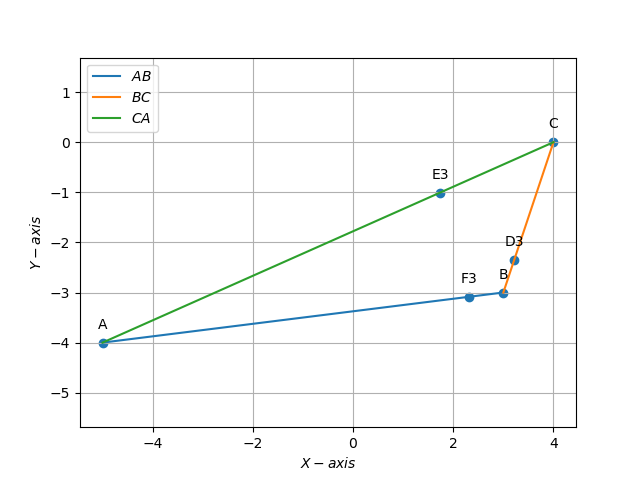
\includegraphics{figs/D3E3F3.png}
    \caption{Points D3 ,E3 ,F3}
    \label{fig:Ang_bisect1}
\end{figure}

 %Question 1.5.3
\item Find the circumcentre and circumradius of $\triangle \vec{D_3E_3F_3}$.  These are the {\em incentre} and {\em inradius} of $\triangle \vec{ABC}$. \\
\solution 
Given\\ 
\begin{align}
    \vec{D_3} &= \myvec{3.21751373 \\ -2.34745882} \\
    \vec{E_3} &= \myvec{1.7388292 \\ -1.0049648} \\
    \vec{F_3} &= \myvec{2.31747277 \\ -3.0853159 } 
\end{align}
\begin{enumerate}
\item For circumcentre :\\
Vector equation of $\vec{D-E}$ is
\begin{align}
(\vec{D_3}-\vec{E_3})^\top\brak{ \vec{x} - \frac{\vec{D_3}+\vec{E_3}}{2}} = 0 \\
(\vec{D_3}-\vec{F_3})^\top\brak{ \vec{x} - \frac{\vec{D_3}+\vec{F_3}}{2}} = 0
\end{align}
on Substituting the values of $\vec{D_3}, \vec{E_3}, \vec{F_3}$ and solving We get,
\begin{align}
     \myvec{1.47868 & -1.34249}\vec{x} &= 5.49147 \label{eq:1.5.3.6} \\
     \myvec{0.900040 & 0.73785}\vec{x} &=0.48655 \label{eq:1.5.3.7}
\end{align}
Thus on solving \eqref{eq:1.5.3.6} and \eqref{eq:1.5.3.7} using gauss elimination We get
\begin{align}
    \myvec{1.47868 & -1.34249 & 5.49147 } \\
    \myvec{0.900040 & 0.73785 & 0.48655 } \\
    \therefore \myvec{1&0\\0&1}\vec{x} &= \myvec{2.18209833 \\ -2.00232035}\\
\implies \vec{x}&=\myvec{2.18209833 \\ -2.00232035}
\end{align}
\item The circiumradius is obtained from  $ \vec{r}=\norm{\vec{I}-\vec{D}_3}$
   \begin{align}
       \vec{I}&=\myvec{2.18209833 \\ -2.00232035} \\
       \vec{D_3} &= \myvec{3.21751373 \\ -2.34745882}  \\
       \vec{I - D_3} &= \myvec{-1.0354154 \\0.34513547} \\
 \vec{r}= \norm{\vec{I}-\vec{D_3}}\ &=  \sqrt{\brak{\vec{I}-\vec{D_3}}^{\top}\brak{\vec{I}-\vec{D_3}}} \\
 \vec{r} &= 1.091422715179266
   \end{align}
\end{enumerate}
\begin{figure}[H]
    \centering
    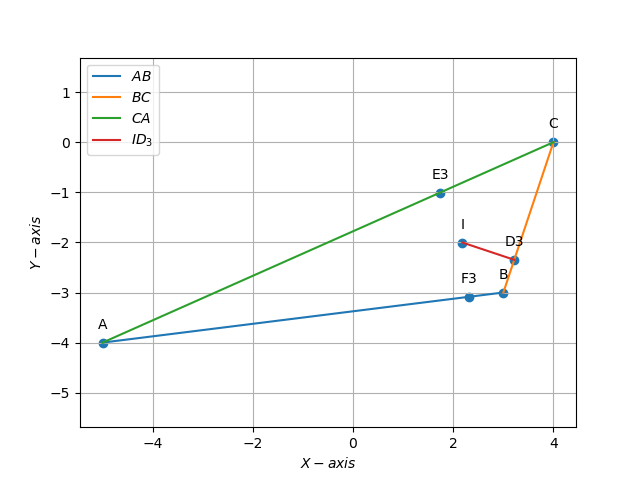
\includegraphics{figs/Incentre_I.png}
    \caption{incentre and inradius of $\triangle ABC$}
    \label{fig:Ang_bisect2}
\end{figure}

 %Question 1.5.4
\item Draw the circumcircle of $\triangle \vec{D_3E_3F_3}$.  This is known as the {\em incircle} of $\triangle \vec{ABC}$. \\
\solution 
\begin{align}
    \vec{D_3} &= \myvec{3.21751373 \\ -2.34745882} \\
    \vec{E_3} &= \myvec{1.7388292 \\ -1.0049648} \\
    \vec{F_3} &= \myvec{2.31747277 \\ -3.0853159 } 
\end{align}
Incentre 
\begin{align}
   \vec{I}&=\myvec{2.18209833 \\ -2.00232035}
\end{align}
Radius
\begin{align}
 \vec{r} &= 1.091422715179266
\end{align}
\begin{figure}[H]
    \centering
    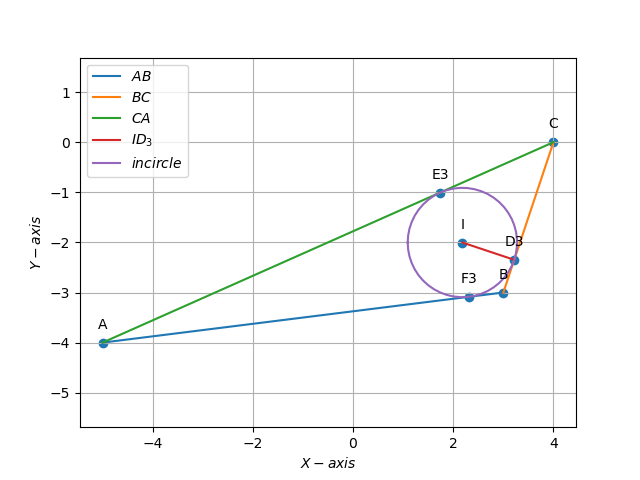
\includegraphics{figs/Incircle.png}
    \caption{incircle of $\triangle ABC$ }
    \label{fig:Ang_bisect3}
\end{figure}


  
 %Question 1.5.5
\item Verify that 
\begin{align}
\angle BAI = \angle CAI.
\end{align}
$AI$ is the bisector of $\angle A$. \\
\solution
\begin{align}
\label{eq:1.5.5.2}
\cos{\angle BAI} \triangleq \frac{(\vec{B}-\vec{A})\top(\vec{I}-\vec{A})}{\norm{\vec{B}-\vec{A}}\norm{\vec{I}-\vec{A}}} \\
\cos{\angle CAI} \triangleq \frac{(\vec{C}-\vec{A})\top(\vec{I}-\vec{A})}{\norm{\vec{C}-\vec{A}}\norm{\vec{I}-\vec{A}}} 
\end{align}
From the given values of $\vec{A},\vec{B},\vec{C}$ and $\vec{I}$,\\
\begin{align}
    \vec{A}=\myvec{-5 \\ -4},\,
    \vec{B}=\myvec{3\\-3},\,
    \vec{C}=\myvec{4\\0},\, \\
    \vec{I}=\myvec{2.18209833 \\ -2.00232035}\\
    \vec{B}-\vec{A} =\myvec{8\\1} \\
    \vec{C}-\vec{A}= \myvec{9\\4} \\
 \vec{I}-\vec{A}=\myvec{7.18209833 \\ 1.99767665}
\end{align}
also calculating the values of norms
\begin{align}
	\norm{\vec{B}-\vec{A}} &= \sqrt{65}\\
	\norm{\vec{C}-\vec{A}} &= \sqrt{97} \\
 	\norm{\vec{I}-\vec{A}} &= 7.454746703 \\
\end{align}

\begin{enumerate}
    \item calculating for $\angle BAI$ : \\
    On substituting the values in  \eqref{eq:1.5.5.2} ,We get 
    \begin{align}
        \cos{\angle BAI} \triangleq \frac{\myvec{ 8 & 1}\myvec{7.18209833 \\ 1.99767665}}{ 
        \sqrt{65}\times 7.4547467039} \\
    \end{align}
    On solving we get,
    \begin{align}
        \angle BAI = 8.4187\degree
    \end{align}
       \item Calculating for $\angle CAI$: \\
    On substituting the values in  \eqref{eq:1.5.5.2} ,We get 
    \begin{align}
        \cos{\angle CAI} \triangleq \frac{\myvec{ 9 & 4}\myvec{7.18209833 \\ 1.99767665}}{ \sqrt{97}\times 7.4547467039 } \\
    \end{align}
    On solving we get,
    \begin{align}
        \angle CAI = 8.4187\degree
    \end{align}
\end{enumerate}
Therefore $\angle BAI = \angle CAI.$ and $AI$ is the bisector of $\angle A$. 
\begin{figure}[H]
    \centering
    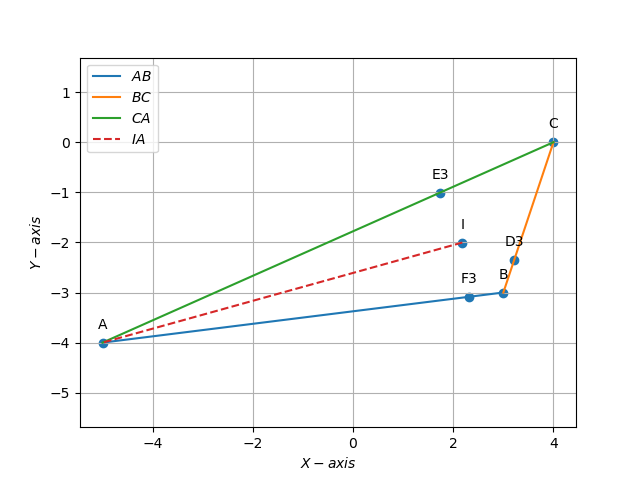
\includegraphics{figs/AI_bisector.png}
    \caption{Angular bisector  $AI$}
    \label{fig:Ang_bisect4}
\end{figure}


%Question 1.5.6
\item Verify that $\vec{BI}, \vec{CI}$ are also the angle bisectors of $\triangle \vec{ABC}$. \\
\solution
\begin{enumerate}
    \item To prove $BI$ is an angular bisector of $ \angle B$
\begin{align}
\label{eq:1.5.6.1}
\cos{\angle ABI} \triangleq \frac{(\vec{A}-\vec{B})\top(\vec{I}-\vec{B})}{\norm{\vec{A}-\vec{B}}\norm{\vec{I}-\vec{B}}} \\
\cos{\angle CBI} \triangleq \frac{(\vec{C}-\vec{B})\top(\vec{I}-\vec{B})}{\norm{\vec{C}-\vec{B}}\norm{\vec{I}-\vec{B}}} 
\end{align}
From the given values of $\vec{A},\vec{B},\vec{C}$ and $\vec{I}$,\\
\begin{align}
    \vec{A}=\myvec{-5 \\ -4},\,
    \vec{B}=\myvec{3\\-3},\,
    \vec{C}=\myvec{4\\0},\, \\
    \vec{I}=\myvec{2.18209833 \\ -2.00232035}\\
	\vec{A}-\vec{B} =\myvec{-8\\-1} \\
	\vec{C}-\vec{B} = \myvec{1\\3} \\
 \vec{I}-\vec{B} =\myvec{-0.81790167 \\ 0.99767665}
\end{align}
also calculating the values of norms
\begin{align}
	\norm{\vec{A}-\vec{B}} &= \sqrt{65}\\
	\norm{\vec{C}-\vec{B}} &= \sqrt{10} \\
 	\norm{\vec{I}-\vec{B}} &= 1.290085982 \\
\end{align}


\begin{enumerate}[label=(\alph*)]
    \item calculating for $\angle ABI$ : \\
    On substituting the values in  \eqref{eq:1.5.6.1} ,We get 
    \begin{align}
        \cos{\angle ABI} \triangleq \frac{\myvec{ -8 & -1}\myvec{-0.81790167 \\ 0.99767665}}{ \sqrt{65}\times 1.290085982} \\
    \end{align}
    On solving we get ,
    \begin{align}
        \angle ABI =57.7998 \degree
    \end{align}
    
       \item calculating for $\angle CBI$: \\
    On substituting the values in  \eqref{eq:1.5.6.1} ,We get 
    \begin{align}
        \cos{\angle CBI} \triangleq \frac{\myvec{ 1 & 3}\myvec{ -0.81790167 \\ 0.99767665}}{ \sqrt{10} \times 1.290085982} \\
    \end{align}
    On solving 
    \begin{align}
        \angle CBI = 57.7998\degree
    \end{align}
    Therefore $\angle ABI = \angle CBI.$ and $BI$ is the bisector of $\angle B$. 
\end{enumerate}


    \item To prove $CI$ is an angular bisector of $ \angle C$
\begin{align}
\label{eq:1.5.6.18}
\cos{\angle BCI} \triangleq \frac{(\vec{B}-\vec{C})\top(\vec{I}-\vec{C})}{\norm{\vec{B}-\vec{C}}\norm{\vec{I}-\vec{C}}} \\
\cos{\angle ACI} \triangleq \frac{(\vec{A}-\vec{C})\top(\vec{I}-\vec{C})}{\norm{\vec{A}-\vec{B}}\norm{\vec{I}-\vec{C}}} 
\end{align}
From the given values of $\vec{A},\vec{B},\vec{C} and \vec{I}$,\\
\begin{align}
    \vec{A}=\myvec{-5 \\ -4},\,
    \vec{B}=\myvec{3\\-3},\,
    \vec{C}=\myvec{4\\0},\, \\
    \vec{I}=\myvec{2.18209833 \\ -2.00232035}\\
    \vec{B}-\vec{C} =\myvec{-1\\-3} \\
    \vec{A}-\vec{C} = \myvec{-9\\-4} \\
    \vec{I}-\vec{C} =\myvec{-1.81790167 \\ -2.0023235}
\end{align}
also calculating the values of norms
\begin{align}
	\norm{\vec{B}-\vec{C}} &= \sqrt{10} \\
	\norm{\vec{A}-\vec{C}} &= \sqrt{97} \\
 	\norm{\vec{I}-\vec{C}} &= 2.704452972 \\
\end{align}

\begin{enumerate}[label=(\alph*)]
    \item calculating for $\angle BCI$ : \\
    On substituting the values in  \eqref{eq:1.5.6.18} ,We get 
    \begin{align}
        \cos{\angle BCI} \triangleq \frac{\myvec{ -1 & -3}\myvec{-1.81790167 \\ -2.0023235}}{ \sqrt{10} \times 2.704452972 } \\
    \end{align}
    On solving we get ,
    \begin{align}
        \angle BCI = 23.8013726 \degree
    \end{align}
       \item similarly for $\angle ACI$ : \\
    On substituting the values in  \eqref{eq:1.5.6.18} ,We get 
    \begin{align}
        \cos{\angle ACI} \triangleq \frac{\myvec{ -9 & -4}\myvec{-1.81790167 \\ -2.0023235}}{ \sqrt{97} \times 2.704452972} \\
    \end{align}
    On solving we get ,
    \begin{align}
        \angle ACI = 23.8013726\degree
    \end{align}
    Therefore $\angle BCI = \angle ACI.$ and $CI$ is the bisector of $\angle C$. 
\end{enumerate}
\begin{figure}[H]
    \centering
     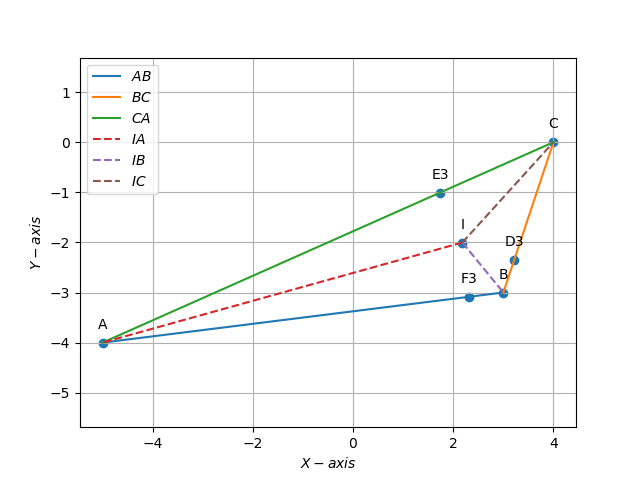
\includegraphics{figs/BICI_bisectors.png}
    \caption{Angular bisectors  $BI$ and $CI$}
    \label{fig:Ang_bisect5}
\end{figure}
\end{enumerate}
All the codes for this section are available at
\begin{lstlisting}
	geometry/Triangle/Angle_bisector/codes/All_AngleBisectors.py
\end{lstlisting}
\end{enumerate}
\end{document}
